\chapter{\texorpdfstring{$N$}{N}-Particles}
\label{ch:np}

In this chapter, we will generalize the system from Chapter \ref{ch:sp} to $N$-particles.
For this, we will consider the same setup as in the 1-Particle case,
    but instead of a single particle and an optical tweezers,
    we consider $N$ Particles with $N$ optical tweezers arranged along the $y$-Axis.
A sketch of the setup can be seen in Figure \ref{fig:np:sketch}
\begin{figure}[!h]
    \centering
    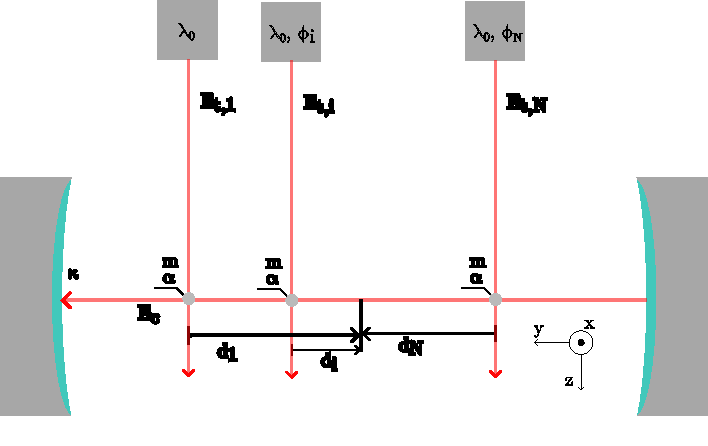
\includegraphics[width=0.8\linewidth]{chapters/11_n_particles/sketch-multi.pdf}
    \caption{
        Setup for $N$-particles \\
        Here we have $N$-Lasers of wavelength $\lambda_0$ and a relative phase $\phi_i$. On the sides are the optical mirrors and at the focal point of each laser is a particle.
    }
    \label{fig:np:sketch}
\end{figure}
\section{Adapting the Modeling}

A lot of the formalism can be carried over
    from the $1$-Particle case.
To get the correct Hamiltonian, 
    we must sum all kinetic terms 
    and all dipole interactions.
There is still only a single Cavity,
    and from that $H_C$ will remain unchanged.
\begin{equation}
    H = 
        \sum_i \left[ \frac{\norm{\vec p_i^2}}{2m_i} 
        - \frac{1}{2}\alpha_i \norm{\vec E_{tot}(\vec r_i)}^2 
        \right]
        + \hbar\omega_c a_c^* a_c
\end{equation} with
\begin{align}
    \vec E_{tot}(\vec r) = \vec E_c(\vec r) + \sum_i \vec\varepsilon_i(\vec r) .
\end{align}


We assume all optical tweezers $\vec\varepsilon_i(\vec r)$ to be modeled by the same Gaussian as in the $1$-Particle case.
Each optical tweezers gains two additional degrees of freedom,
    the position along the $y$-axis can be varied, which we will call $\vec R_i = d_i \vec e_y$
    and the phase, which we will denote with $\varphi_i$.
We also assume that the rest of the parameters are assumed to be equivalent.
With this, we write our new tweezers as
\begin{align}
    \label{eq:np:model:epsi}
    \vec \varepsilon_i(\vec r) = \vec e_x \left[ E_{t,i}(\vec r)\exp(-\i\omega_0t) + c.c. \right]\\ 
    \quad\quad E_{t,i}(\vec r) = E_t\left(\vec r-\vec R_i\right)\exp(\i\varphi_i).
\end{align}
Since any global phase is not detectable,
    we may choose $\varphi_1 = 0$ without loss of generality.

To make the modeling easier, 
    we assume that the distances between the intensity maximums of the tweezers satisfy $|d_i - d_j| \gg W_t~\forall~1\leq i,j <N,i\neq j$,
    such that the optical tweezers only act on their respective particle.
Due to this approximation, the particles will only couple through the cavity field
    and have no interaction otherwise.
Under this assumption, the total electric field becomes
\begin{equation}
    \vec E_{tot}(\vec r_i) \approx E_c(\vec r_i) + \vec \varepsilon_i(\vec r_i).
\end{equation}

Time averaging the system simplifies our Hamiltonian, 
    in complete analogy to the $1$-Particle case, we get
\begin{equation}
\begin{split}
    H = &-\sum_i  \left[
         \frac{\alpha}{2} \left[ 
            |E_{t,i}(\vec r_i)|^2 
            + E_c^2(\vec r_i)  a_c^* a_c + \left[ 
                E_c(\vec r_i) E_{t,i}^*(\vec r_i) a_c \exp(\i\omega_0t) + c.c. 
            \right]
        \right]
    \right] \\
       &+\sum_i\frac{1}{2m} \norm{\vec p_i}^2 + \hbar\omega_c a_c^* a_c.
\end{split}
\end{equation}

\section{Equations of Motion}

This Hamiltonian can be used to get the time evolution of $a_c$
\begin{equation}
\dot a_c = -\i \left( \omega_c - \frac\alpha\hbar \sum_i E_c^2(\vec r_i)\right)a_c + \frac{\i\alpha}\hbar \sum_iE_c(\vec r_i)E_{t,i}(\vec r_i) \exp(-\i\omega_0 t).
\end{equation}

The same transformation as with the $1$-Particle case can be used to remove the explicit time dependence.
Setting the time derivative to zero and simplifying yields
\begin{equation}
    \alpha_c^{eq} = \frac\alpha\hbar \frac{\sum_i E_c(\vec r_i) E_{t,i}(\vec r_i)}{\omega_c-\omega_0-\frac\alpha\hbar \sum_i E_c^2(\vec r_i)}.
\end{equation}
Damping needs to be added the same way by adding a term of $- i\kappa/2$ to the denominator.
Similarly to the $1$-Particle case we also define 
\begin{equation}
    \delta_c := \omega_c - \omega_0 - \frac\alpha\hbar \sum_i E_c^2(\vec r_i) = \Delta - \frac\alpha\hbar \sum_i E_c^2(\vec r_i).
\end{equation}

Which gives almost the same form as the $1$-Particle case
\begin{equation}
    \alpha_c^{eq} = \frac\alpha\hbar \frac{\sum_i E_c(\vec r_i) E_{t,i}(\vec r_i)}{\delta_c - i\frac{\kappa}{2}}
\end{equation}

The new condition for stability is
\begin{equation}
    \dot{\vec p_i} 
        = -\grad_{i} H 
        = + \alpha \grad_i|\alpha_c E_c(\vec r_i) + E_{t,i}(\vec r_i)|^2 \overset{!}{=}\vec 0.
\end{equation}
$\grad_i$ being the spatial derivative of the $i$-th Particle.

\section{Finding the Extremes}
\label{sec:np:extrem}

We will use logarithmic gradients again.
The definition for $\vec g$ does not change and can simply be reused from Section \ref{sec:sp:extrem}.
The definition for $\vec f$ needs to be adapted to be
\begin{equation}
    \vec f_i(\vec r_i) := \grad_i \ln E_{t,i}(\vec r_i) 
    \Leftrightarrow \grad_i E_{t,i}(\vec r_i) = \vec f_i(\vec r_i) E_{t,i}(\vec r_i)
    \Leftrightarrow \vec f_i(\vec r_i) = \vec f(\vec r_i-\vec R_i).
\end{equation}

We use the property of $\partial |f|^2 = 2\Re\{f^*\partial f\}$ to get the equilibrium condition
\begin{equation}
\label{eq:np:extrem:cond}
    2\Re\left\{ 
        \left[ \alpha_c^* E_c(\vec r_j) + E_{t,j}(\vec r_j) \right]
        \left[ \alpha_c \vec g(\vec r_j)E_c(\vec r_j) + \vec f_j(\vec r_j) E_{t,j}(\vec r_j) \right] 
    \right\} \overset{!}{=} 0.
\end{equation}

Since we introduced more complex degrees of freedom, 
    we cannot simplify this expression further.
However, this form is already sufficient to analyze its components,
    which we will do in the following sections.

\subsection{\texorpdfstring{$x$}{x}-Component}
\label{ssec:np:extrem:x}

Based on the definitions in Equations \eqref{eq:np:model:epsi} and \eqref{eq:sp:Ec}, 
    the logarithmic gradients for the $x$ component are
\begin{align}
    f_{x,j}( \vec r_j) &= x \left[\i \frac{k_0z_j}{z_j^2 + z_R^2} - \frac{2}{A_x^2 W^2(z_j)}\right] 
\end{align}
and
\begin{align}
    g_x( \vec r_j) &= -\frac{2x_j}{W_c^2} .
\end{align}

In the second multiplicative term, 
    we can factor out an $x_j$
\begin{equation}
   x_j \left[ 
        -\alpha_c \frac{2}{W_c^2}E_c(\vec r_j) 
        + \left[\i \frac{k_0z_j}{z_j^2 + z_R^2} 
        - \frac{2}{A_x^2 W^2(z_j)}\right]E_{t,j}(\vec r_j) 
    \right] .
\end{equation}
Since $x_j$ is real, it can be factored out of the $\Re$ operation 
    and the condition is satisfied by $x_j = 0$.
Which also can be expected since in the $1$ particle case, 
    the solution was $x = 0$ independent of $y$ and $z$
    and the shift does not affect the $x$ direction in any way.


\subsection{\texorpdfstring{$y$}{y}-Component}
\label{ssec:np:extrem:y}

Based on the definitions in Equations \eqref{eq:np:model:epsi} and \eqref{eq:sp:Ec},
    the logarithmic gradients are
\begin{align}
    f_{y,j}( \vec r_j) &= (y_j-d_j) \left[ \i\frac{k_0z_j}{z_j^2+z_R^2} - \frac{2}{A_y^2 W^2(z_j)}\right]
\end{align}
and
\begin{align}
g_y(\vec r_j) &= - k_c\tan(k_c y) 
    %= -k_c \left[ \tan(k_cd_j)  + \tan'(k_cd_j) (y_j-d_j) + \O\left((y_j-d_j)^2\right)\right].
\end{align}

If we require $y_i = d_i$ and $\tan k_c y_i = 0$, both $f_{y, i}$ and $g_y$ are zero.
Substituting this into the second multiplicative term in Equation \eqref{eq:np:extrem:cond} gives
\begin{equation}
  \left[ 0 \cdot \alpha_c E_c(\vec r_j) + 0\cdot E_{t,j}(\vec r_j) \right] {=} 0,
\end{equation}
which also immediately satisfies the condition.

With this, we can conclude that the particle will stay at $y_i - d_i = 0$ if $\tan k_c d_i =0 $ is satisfied. 
This condition adds a constraint on where we can place the tweezers.
For this thesis, we will only consider cases
    where this condition is satisfied.

\subsection{\texorpdfstring{$z$}{z}-Component}
\label{ssec:np:extrem:z}
To simplify this condition, 
    we use the previous conditions.
    ($x = 0$ and $y_i = d_i$)
Under those, we can write the special cases of our tweezers field as
\begin{align}
    E_{t,i}(\vec r_i) = E_t(z \vec e_z) \exp(\i\phi_i).
\end{align}
This gives us the logarithmic gradients in $z$ as
\begin{align}
    f_{z,j}(\vec r_j) 
        & = f_{z}(z_j \vec e_z) 
        = \left[ 
            \i\left( k_0-\frac{z_R}{z_j^2 + z_R^2} \right) - \frac{z_j}{z_j^2 + z_R^2} 
        \right]
\end{align}
and
\begin{align}
    g_z(\vec r_j) &= -\frac{2z_j}{W_c^2}.
\end{align}

We may substitute this finding into Equation \eqref{eq:np:extrem:cond}, 
    and we get a condition that depends on the particle positions in $z_j$.
Note that since we assumed the tweezers would not affect each other,
    the coupling to the other particle positions originates only from the equilibrium condition of the cavity field $\alpha_{c}^{eq}(z_1,z_2,...,z_N)$.

For $N$ particles, we get $N$ coupled conditions.
We can gather all of those conditions
    and write them as one multi variable problem.
To do this, we define
    \begin{equation}
        \vec L(z_1,z_2,..., z_N) = \vec L(\vec z) = 0,~\vec L: \R^N \rightarrow \R^N
    \end{equation}
with each component representing the partial derivative of a different particle's position,
    or written as a formula
\begin{align}
    L_i(\vec z) &:= \alpha \grad_i|\alpha_c^{eq} E_c(\vec r_i) + E_{t,i}(\vec r_i)|^2 \\
    & =  2\alpha\Re\left\{ 
        \left[ \alpha_c^{eq*} E_c(\vec r_i) + E_{t,i}(\vec r_i) \right]
        \left[ \alpha_c^{eq} g_z(\vec r_i)E_c(\vec r_i) + f_{z,i}(\vec r_i) E_{t,i}(\vec r_i) \right] 
    \right\}.
\end{align}

\section{Numerical Computation}

For the numeric computation, we use the Package \pkg[4.5.1]{NLsolve.jl},
    with a trust region Newton style algorithm as described by \textcite{DennisJ.E1983Nmfu}. 
This method reduces divergence to $\infty$ for the solutions,
    which is prone to happen using the standard Newton algorithm.


Similar to the standard Newton algorithm, 
    this method requires starting guesses.
For those, we use the $N$-fold Cartesian product of the solutions obtained from the $1$ particle case.
This works since we assume the particle positions to be similar to those solutions.
To improve the coverage of our method,
    we consider both the positive solutions 
    and mirror them to the negative axis.
Mathematically, the starting guesses can be written as
\begin{align}
    \mathcal{Z}_i &=\{z\quad |L_z(z) = 0\} \\
    \mathcal{Z} &= \mathcal{Z}_1 \otimes \mathcal{Z}_2\otimes ... \otimes\mathcal{Z}_N\equiv \mathcal{Z}^N_i.
\end{align}
Alternatively, one may choose a very fine grid,
    which is very computationally heavy, 
    since the number of starting points scales with the $N$-th power.

Using those results, we can begin to look at special values of $N$. 
In the next chapter, we will find the equilibrium positions of $2$ particles.
For the calculation, we used the same parameters in Table \ref{tab:sp:sim:params}.
Additionally, we kept $\kappa = 180 ~2\pi \unit{kHz}$.
All roots we compute are determined to be $0$ in the error range of the numerical precision.